\chapter{GEM Detector Data Analysis}

Gas Electron Multiplier (GEM) detector is one kind of gaseous detector. At the heart of these detectors is a 5 µm copper-coated polyimide foil, which is punctured with 70 µm holes in a regular hexagonal pattern, spaced 140 µm apart. The GEM foil features a cathode on top, while a readout board is situated beneath it for collecting the electrons generated during the ionization process. When a potential difference is applied across the foils, it produces sharp electric fields within the holes, which multiply the electrons and result in an electron avalanche. This avalanche electrons travels along the electric field and is eventually collected by the finely spaced strips. To enhance amplification, multiple GEM detector layers are stacked together, allowing ionized electrons to be amplified multiple times before reaching the readout board.

The GEM detectors utilized in the PRex/CRex experiment were specifically designed for the Jefferson Lab Super BigBite Spectrometer (SBS) and span an area of 50 cm x 60 cm. At the time of its construction, it was one of the largest GEM detectors ever built. The PRex/CRex experiment offered an excellent opportunity to test the GEM detector in a real experimental environment before initiating the SBS experiment. The detector serves as a valuable supplement in situations where the event rate is high, as the VDC efficiency declines or even fails under such conditions. This chapter delves into the apparatus and the analysis results of the GEM detectors.

\section{GEM Detector Configuration}

The SBS GEM detector used in the PRex/CRex experiment comprises three layers of GEM foils. The cathode, situated on top of the GEM foil, features a similar hole structure but is single-side coated instead of double-sided. To prevent polarization due to charge accumulation on the cathode, a thin aluminized gas window layer is applied, which shares the same high voltage as the cathode.

A premixed gas containing $75\%$ Argon and $25\%$ Carbon Dioxide is supplied by the Hall A gas system for use in the GEM detector. This mixed gas first enters the chamber between the entrance window and the cathode, then passes through the holes in the foil, ensuring a uniform gas mixture throughout the entire chamber. Exhaust gas exits through exhaust holes located on the frame at the bottom of the GEM chamber.

At the base of the GEM foils, avalanche electrons are collected by 2D readout strips. Each readout strip is connected to a charge-sensitive pre-amplifier electronics channel. To counteract any bending of the readout board due to the mixed gas in the chamber, an additional chamber is designed beneath the readout board and filled with air at the same pressure as the GEM chambers.


\begin{figure}[!tbp]
  \centering
  \begin{minipage}[b]{0.45\textwidth}
    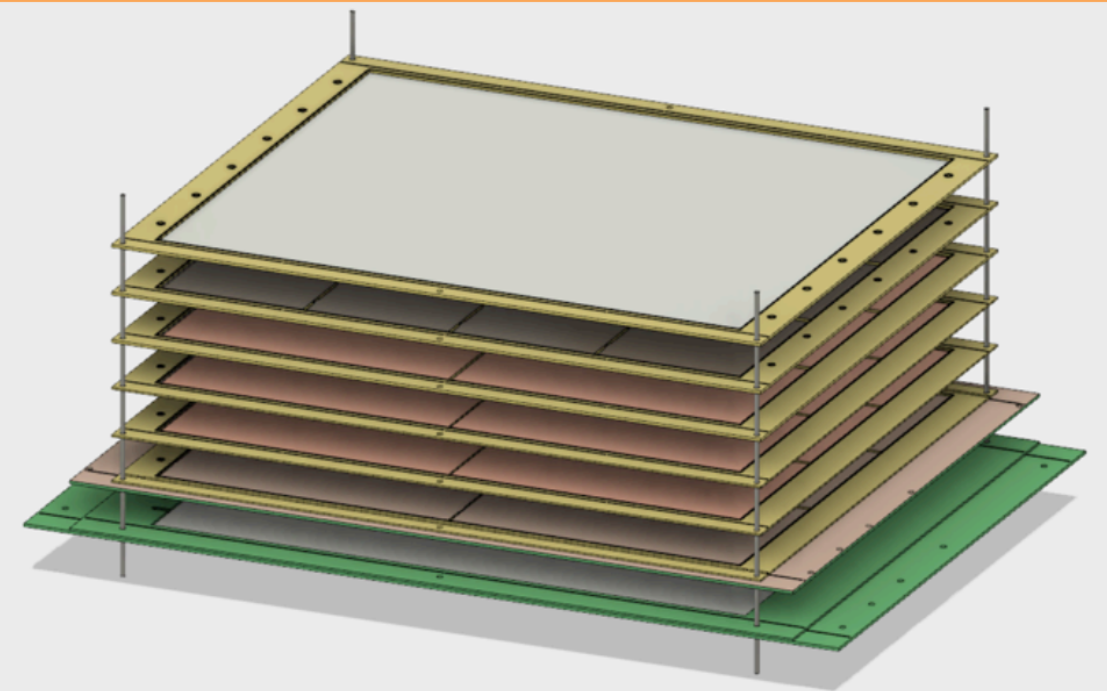
\includegraphics[width=\textwidth]{images/chap5/gem_structure_3d.png}
    \caption{GEM Chamber 2D structure}
  \end{minipage}
  \hfill
  \begin{minipage}[b]{0.45\textwidth}
    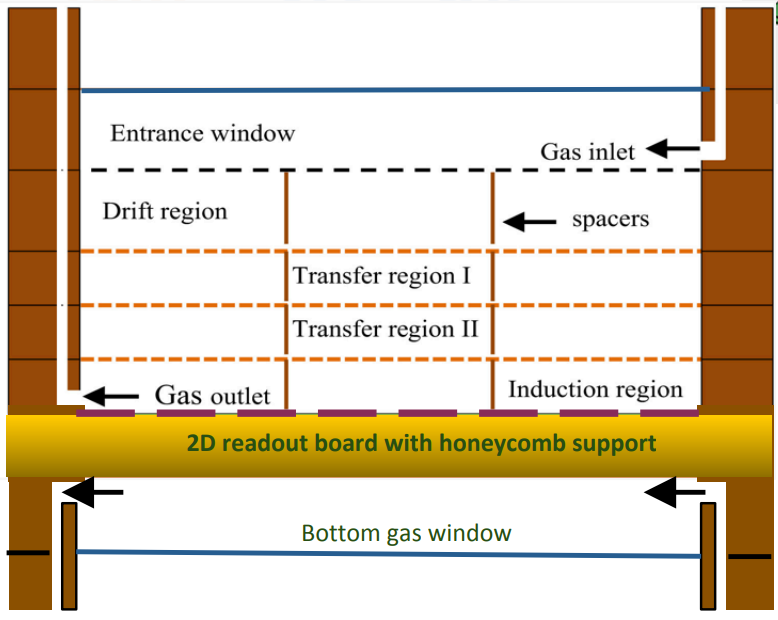
\includegraphics[width=\textwidth]{images/chap5/gem_structure_chamber_2d.png}
    \caption{GEM chamber Gas flow}
  \end{minipage}
\end{figure}


\subsection{GEM Detector in Hall A High-Resolution Spectrometer}

Each High-Resolution Spectrometer (HRS) in Hall A is equipped with three large SBS GEM detectors, each measuring $50 cm \times 60 cm$, and three smaller GEM detectors measuring $10 cm \times 20 cm$ produced by Idaho State University. As depicted in the corresponding figure, the GEM detectors are arranged parallel to each other and placed after the Vertical Drift Chamber (VDC) detectors. The smaller Idaho GEM detectors are positioned in front of the larger SBS GEM detectors. Two quartz detectors are placed between the first and second Idaho GEM detectors, while two AT detectors are situated between the SBS GEM detectors and the Idaho GEM detectors.


\begin{figure}[!htbp]
  \centering
  \begin{minipage}[b]{0.45\textwidth}
    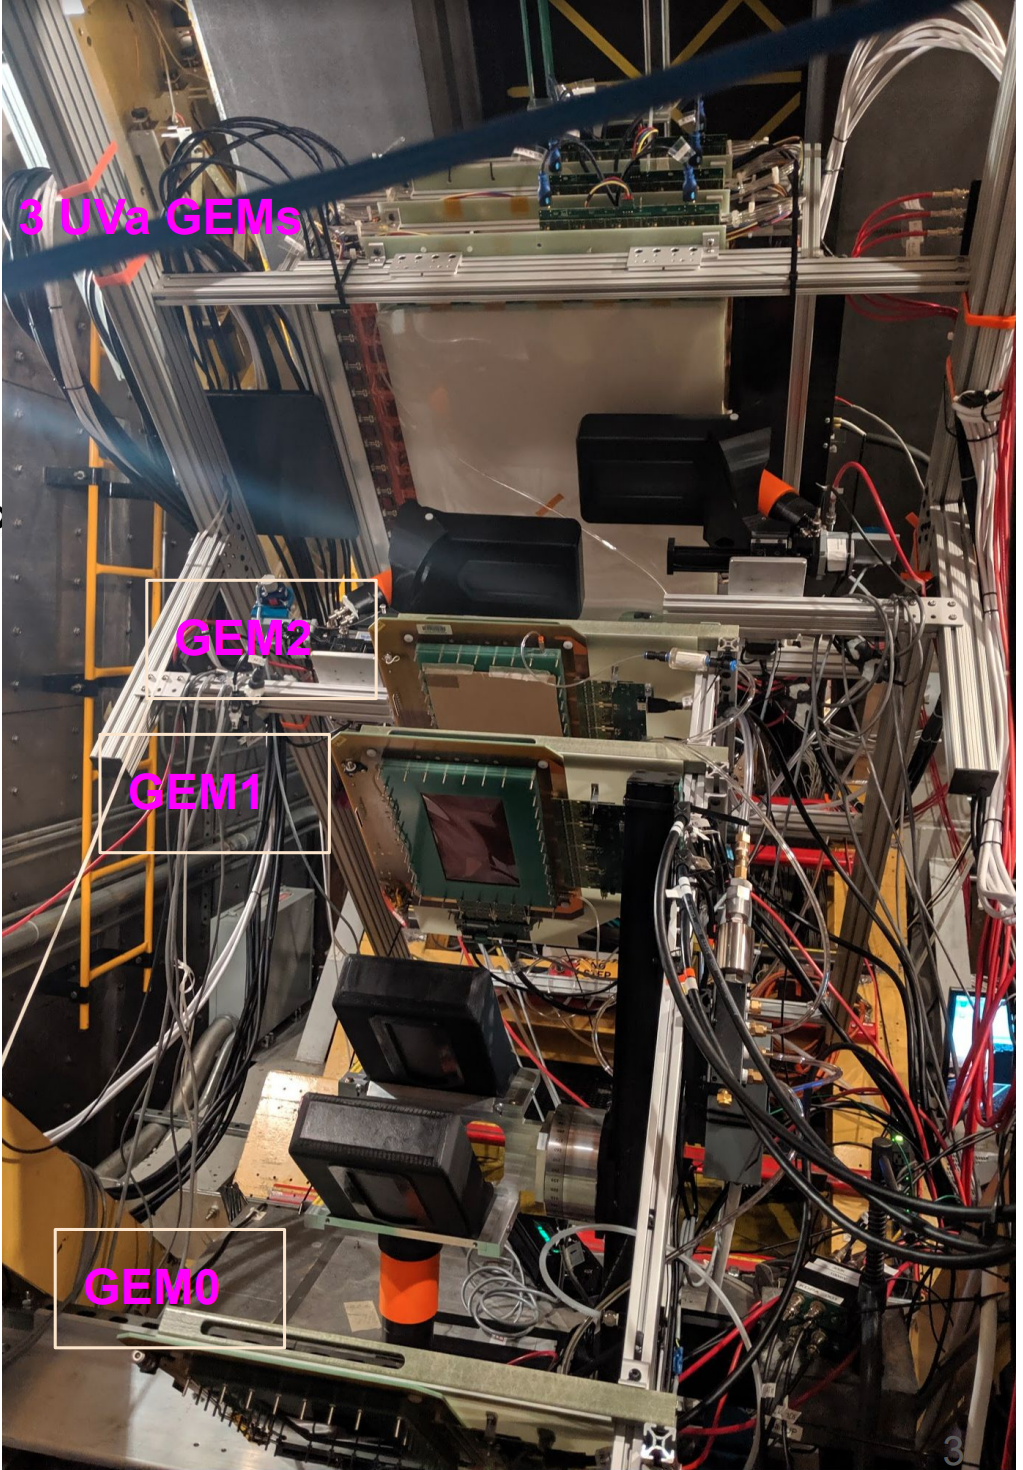
\includegraphics[width=\textwidth]{images/chap5/gem_in_apparatus_photo.png}
    \caption{GEM Chamber 2D structure}
  \end{minipage}
  \hfill
  \begin{minipage}[b]{0.45\textwidth}
    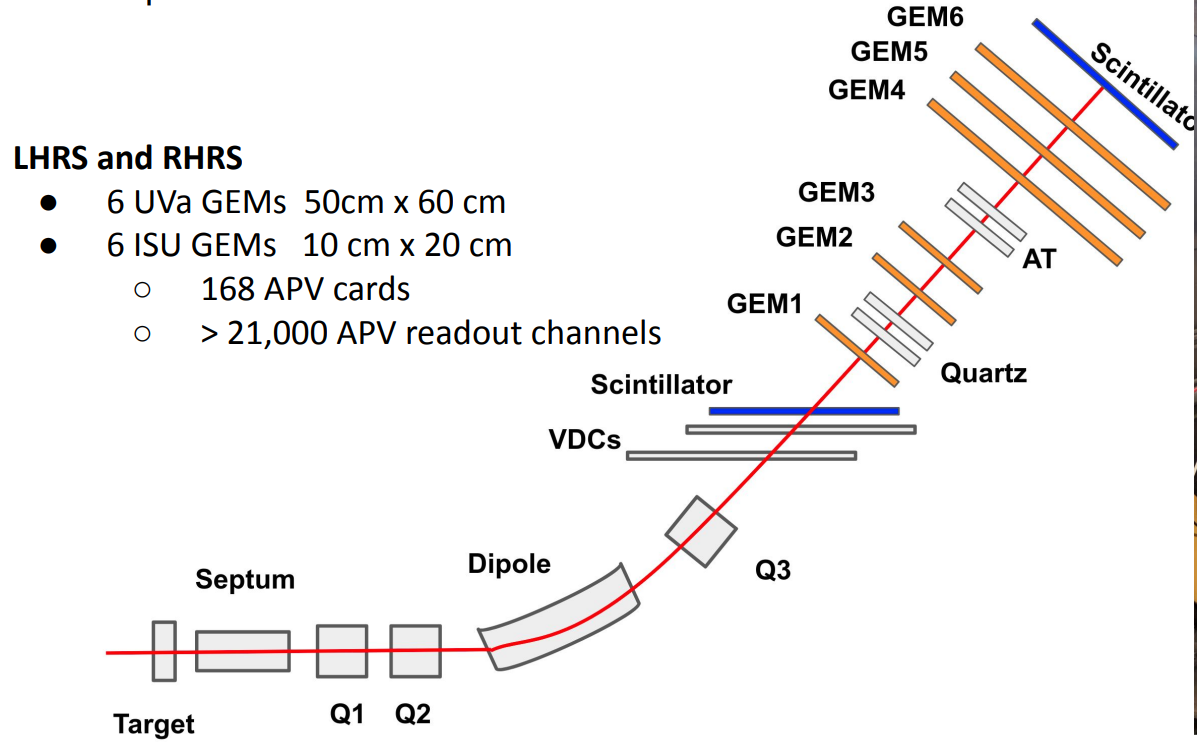
\includegraphics[width=\textwidth]{images/chap5/gem_apparatus_in_hrs_2d.png}
    \caption{GEM chamber Gas flow}
  \end{minipage}
\end{figure}


\subsection{Add a more detailed introduction of GEM detector supplement electronics??}
\begin{enumerate}
    \item readout electronics (APV, MPD, CPU, coda)
    \item low voltage for the APV (modular LV, cable selection, LV regulator, cooling fan) 
    \item High Voltage
    \item Gas System
\end{enumerate}


\begin{figure}[!htbp]
  \centering
  \begin{minipage}[b]{0.45\textwidth}
    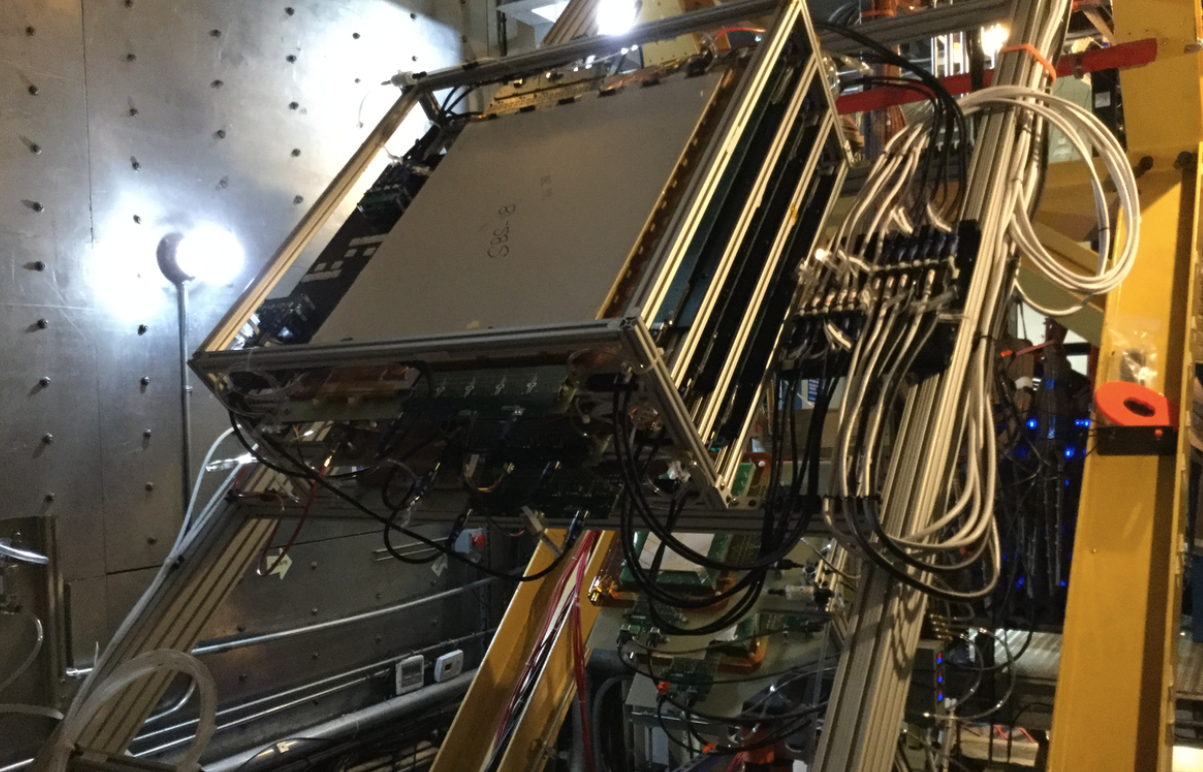
\includegraphics[width=\textwidth]{images/chap5/gem_in_hrs.png}
    \caption{GEM Chamber in HRS}
  \end{minipage}
  \hfill
  \begin{minipage}[b]{0.45\textwidth}
    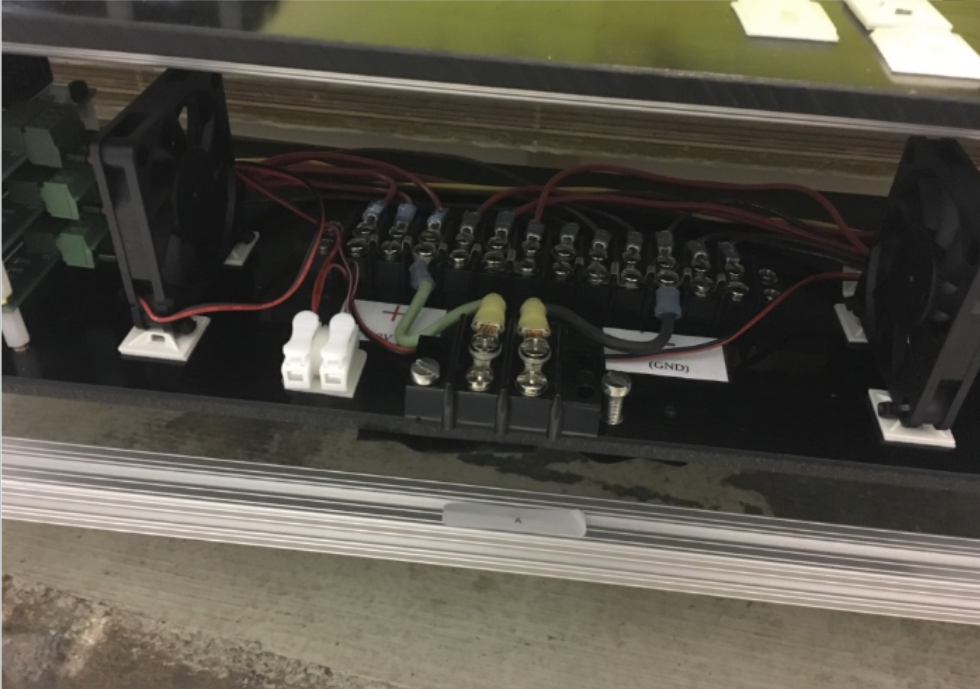
\includegraphics[width=\textwidth]{images/chap5/gem_low_voltage.png}
    \caption{GEM Pre-Amplifier Voltage Supply}
  \end{minipage}
\end{figure}


\begin{figure}
    \centering
    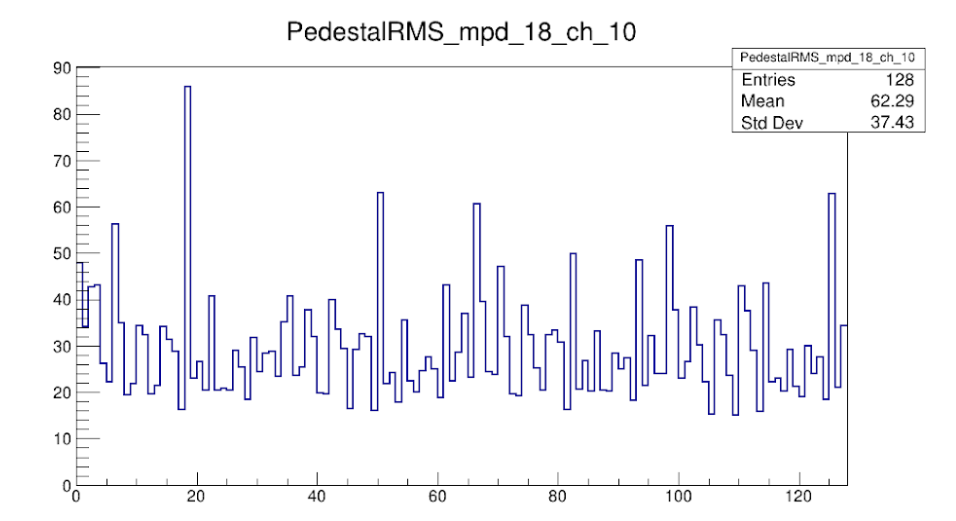
\includegraphics[width=\textwidth]{images/chap5/gem_signal.png}
    \caption{Caption}
    \label{fig:apv_25_pedestal_plot}
\end{figure}

\section{GEM Detector Data Analysis}

The GEM detector readout strips are connected to the APV frontend card, a 128-channel pre-amplifier. The signal from the APV is transmitted to a Multi-Purpose Digitizer, where it is converted to digital signals using a 12-bit Analog to Digital Converter. Figure \ref{fig:apv_25_pedestal_plot} displays a typical plot after MPD conversion. The x-axis represents the APV channels, and the y-axis corresponds to the ADC values after the conversion, which are proportional to the number of charges collected by the given strip.

To extract useful signals, multiple steps are typically employed, including common mode subtraction, pedestal measurement, and fired strips selection.

\subsection{GEM Pedestal Measurement}

A pedestal run involves setting the high voltage to 2000 V for a dry run. At this high voltage, the electric field is insufficient to trigger an avalanche, meaning no signal should be detected on the readout strips. By applying a 2000 V high voltage, the noise from the high voltage modules can be considered when estimating the pedestal, as opposed to having no high voltage applied. The pedestal of each channel of the 128 APV channels is calculated by subtracting the ADC value from the common mode, defined as the average of the 128-channel ADC values. Subsequently, the Root Mean Square (RMS) and mean of each channel's pedestal are computed across all the events that have been recorded.

Figure \ref{fig:lhrs_pedestal_distribution} and \ref{fig:rhrs_pedestal_distribution} show the pedestal distributions of all the channels used in the PRex experiment. The x-axis represents the index of the APV card, and the y-axis corresponds to the RMS value of the pedestal. Each data point in the plot represents one GEM readout channel.

The first 18 APV cards are utilized in the Idaho GEM detectors. As the area of these detectors is $10 cm \times 20 cm$, their pedestal RMS values are also smaller than those of the SBS GEM detectors. The LHRS GEM detectors have larger pedestal RMS values than those of the RHRS, with RMS values of around 20 ADC, which equates to approximately $0.02 V$ voltage fluctuation. A few channels in each APV card exhibit much higher pedestals, and these are considered dead channels due to issues in the Printed Circuit Board (PCB) manufacturing process.

\begin{figure}[!htbp]
    \centering
    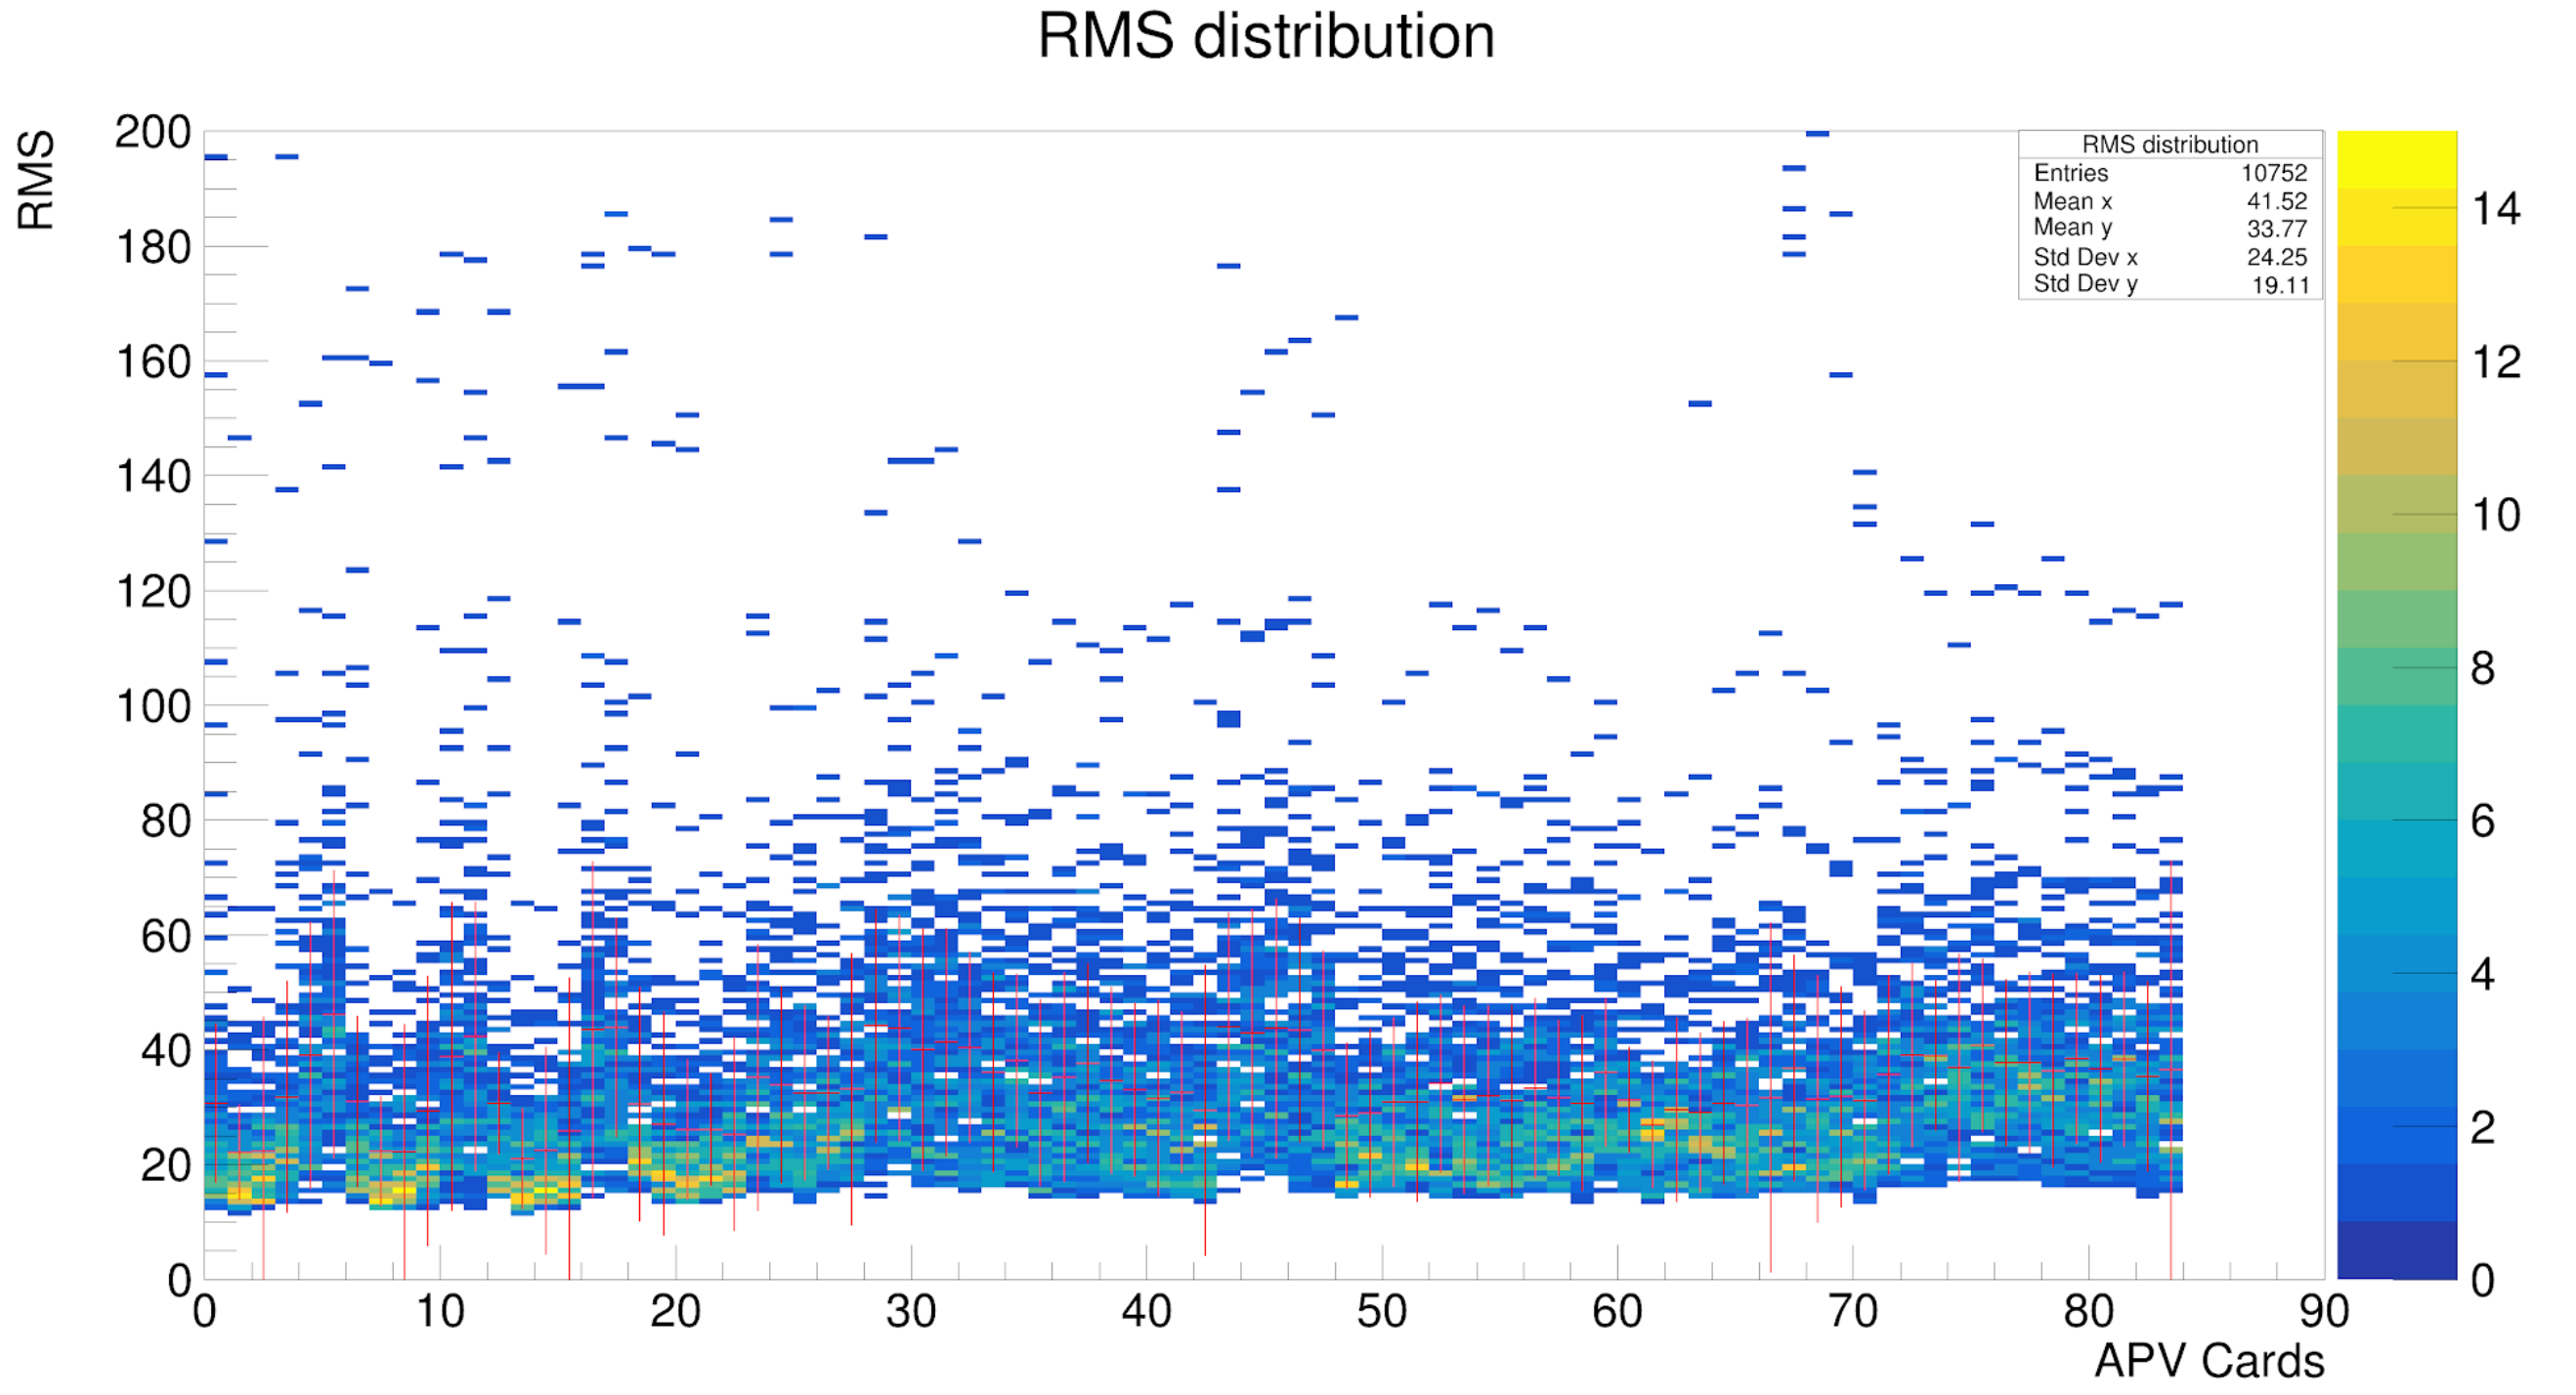
\includegraphics[width=\textwidth]{images/chap5/LHRS_pedestal.png}
    \caption{LHRS GEM Readout RMS of Pedestal Distribution}
    \label{fig:lhrs_pedestal_distribution}
\end{figure}

\begin{figure}[!htbp]
    \centering
    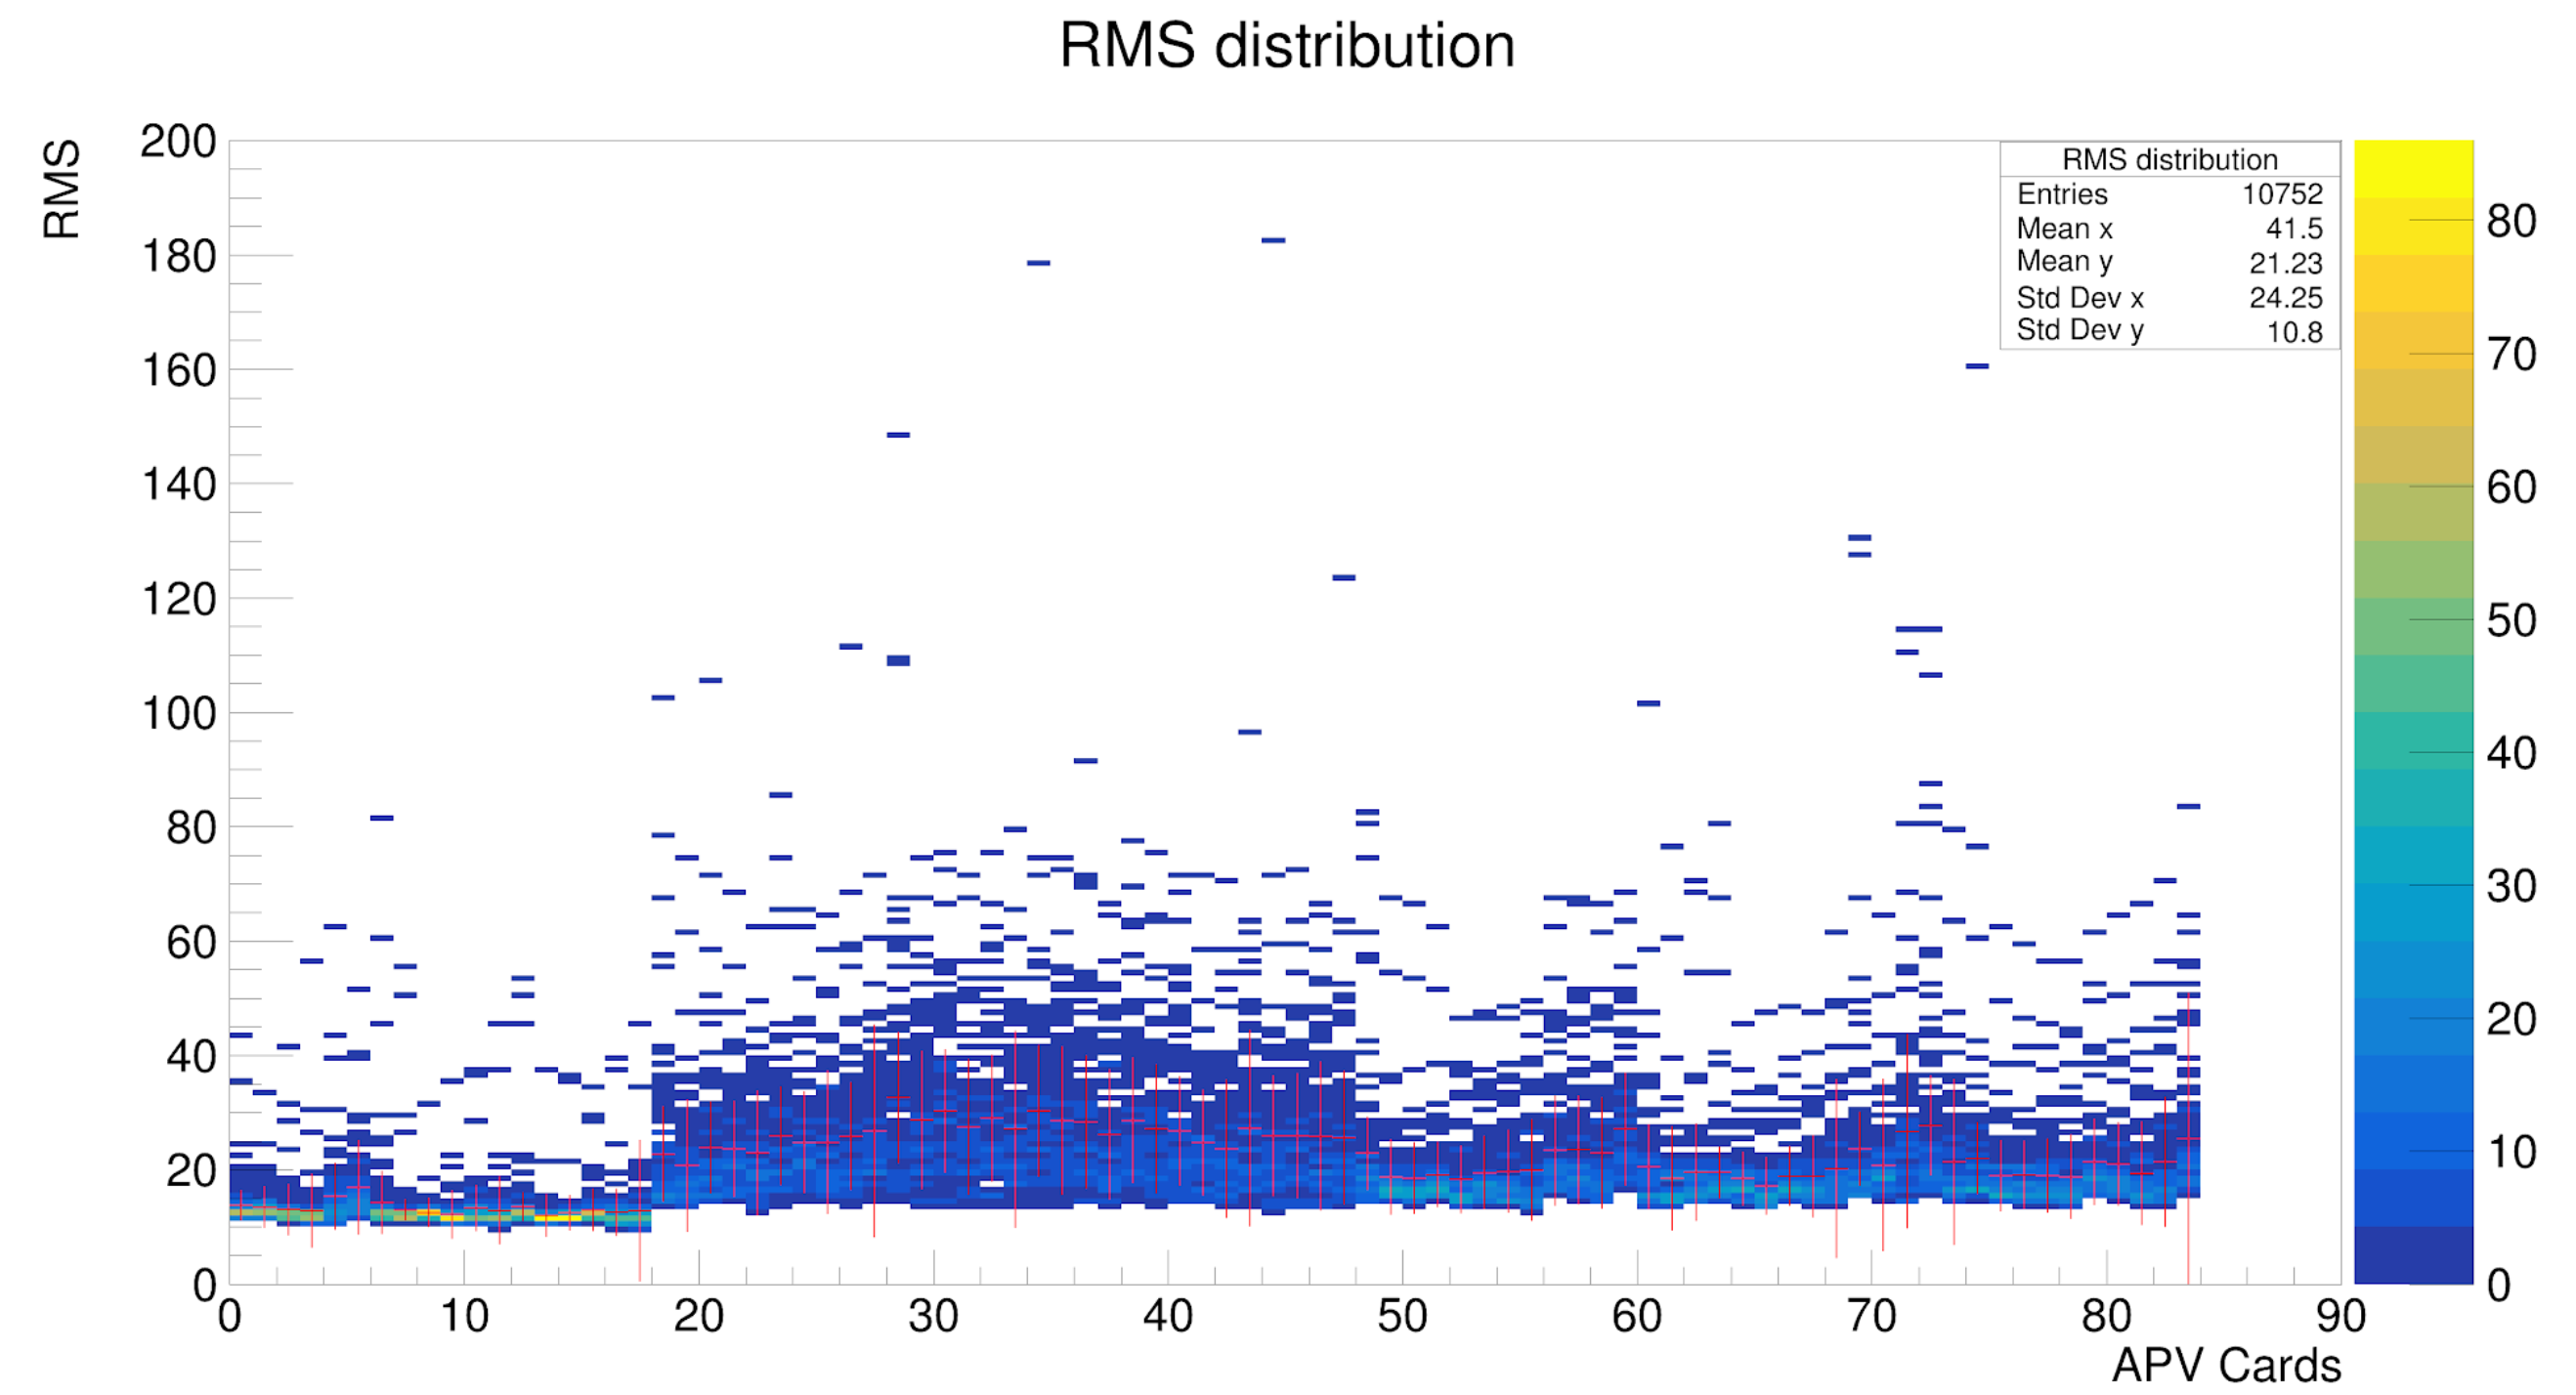
\includegraphics[width=\textwidth]{images/chap5/rhrs_pedestal.png}
    \caption{RHRS GEM Readout RMS of Pedestal Distribution}
    \label{fig:rhrs_pedestal_distribution}
\end{figure}


\subsubsection{GEM detector false positive rate}

When the GEM detector works at Normal working voltage. When a particle passes through  the GEM detectors and ionized the gases inside the GEM chambers. The ionized electrons will travel along the Electric field and get amplified within the holes in GEM detectors, and then the avalanche electrons will be collected by the readout strips and readout with the electronics. 

Similar to the algorithm used for calculating the pedestals, the signals will first subtract the common mode. After that, the value of the strips is calculated by subtracting the value from the corresponding mean of the pedestals. The determination of GEM fired strip is determined by comparing the calculated values with the threshold. Different channels may have different noise performances, to get a consistent criterion, the threshold of given channels is chosen to be n*rms of the pedestal. If the value is larger than the threshold, the given strips are considered to be fired strips. 

If the threshold is too high, there is more chance fired strip to categorized to be non-signal (False Negative), on the other hand, if the threshold is set too low, the is more chance a white noise will be categorized to be fired strips (False Positive). 

To measure the false positive rate, the GEM signal selection algorithm is applied on a 2000v voltage dry run. At 2000v there should no real signals, if there is any triggered strips, those are fake fired signals. By measuring the ratio of the fired strips in the dry run, we can estimate the False Positive Rate of the algorithm. In fig \ref{fig:lhrs_fake_hit_rate} and \ref{fig:rhrs_fake_hit_rate} are the fake hit rate for the SBS GEM detectors on the LHRS and Right HRS. At the $5\sigma$ threshold, the fake hit rate for left HRS is $0.16\%$ and $0.01\%$.

\subsubsection{High Voltage Scan Efficiency for GEM detectors}
\subsubsection{GEM detector number of cluster performance}
\subsubsection{GEM detector cluster size performance}


\begin{figure}[!htbp]
    \centering
    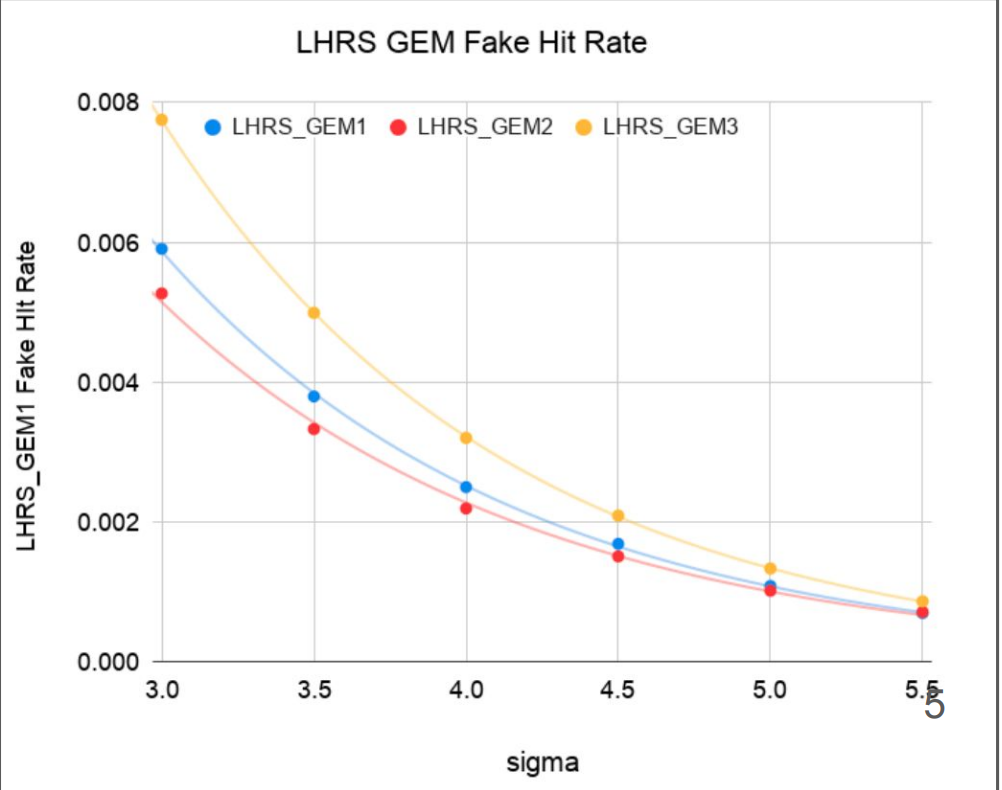
\includegraphics[width=\textwidth]{images/chap5/lhrs_fake_hit_rate.png}
    \caption{LHRS SBS GEM Fake Hit Rate}
    \label{fig:lhrs_fake_hit_rate}
\end{figure}

\begin{figure}[!htbp]
    \centering
    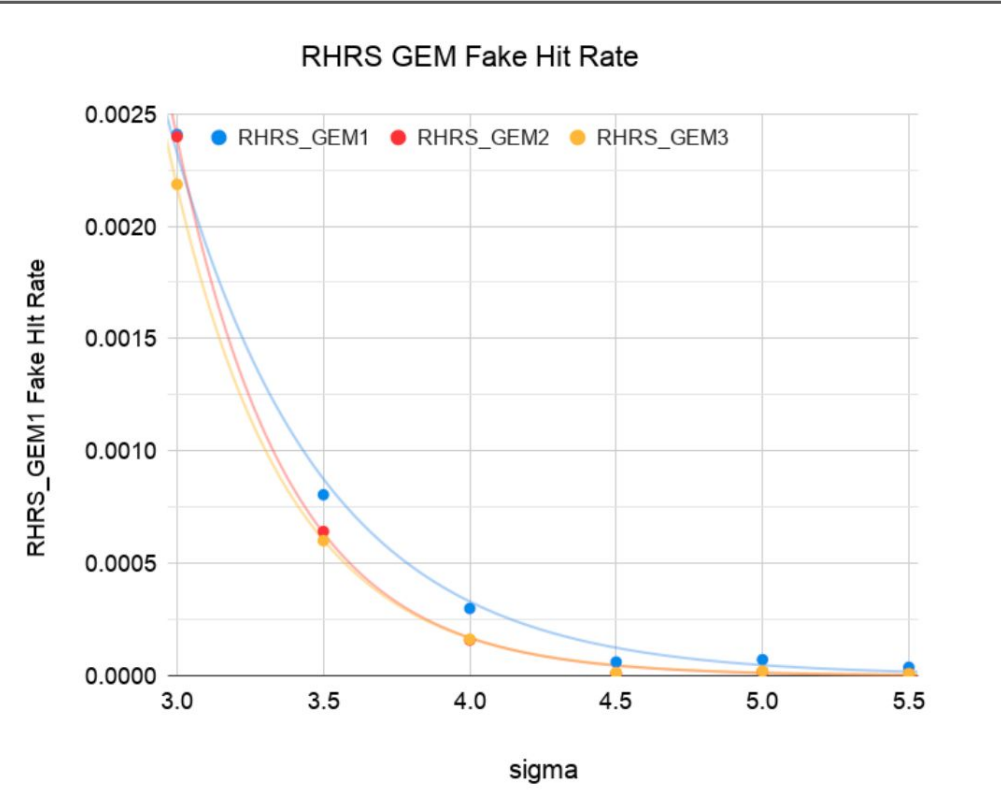
\includegraphics[width=\textwidth]{images/chap5/rhrs_fake_hit_rate.png}
    \caption{RHRS SBS GEM Fake Hit Rate}
    \label{fig:rhrs_fake_hit_rate}
\end{figure}

\subsection{GEM detector alignment}

\subsubsection{tree search algorithm used for search for the GEM cluster}
\subsubsection{Multiple GEM detectors alignment algorithm }
\subsection{GEM detector performance}

\subsubsection{GEM detector efficiency with tracking}
\subsubsection{GEM detector efficiency over time}
\subsubsection{GEM detector High Rate Performance and compare with VDC}

\begin{figure}[!htbp]
    \centering
    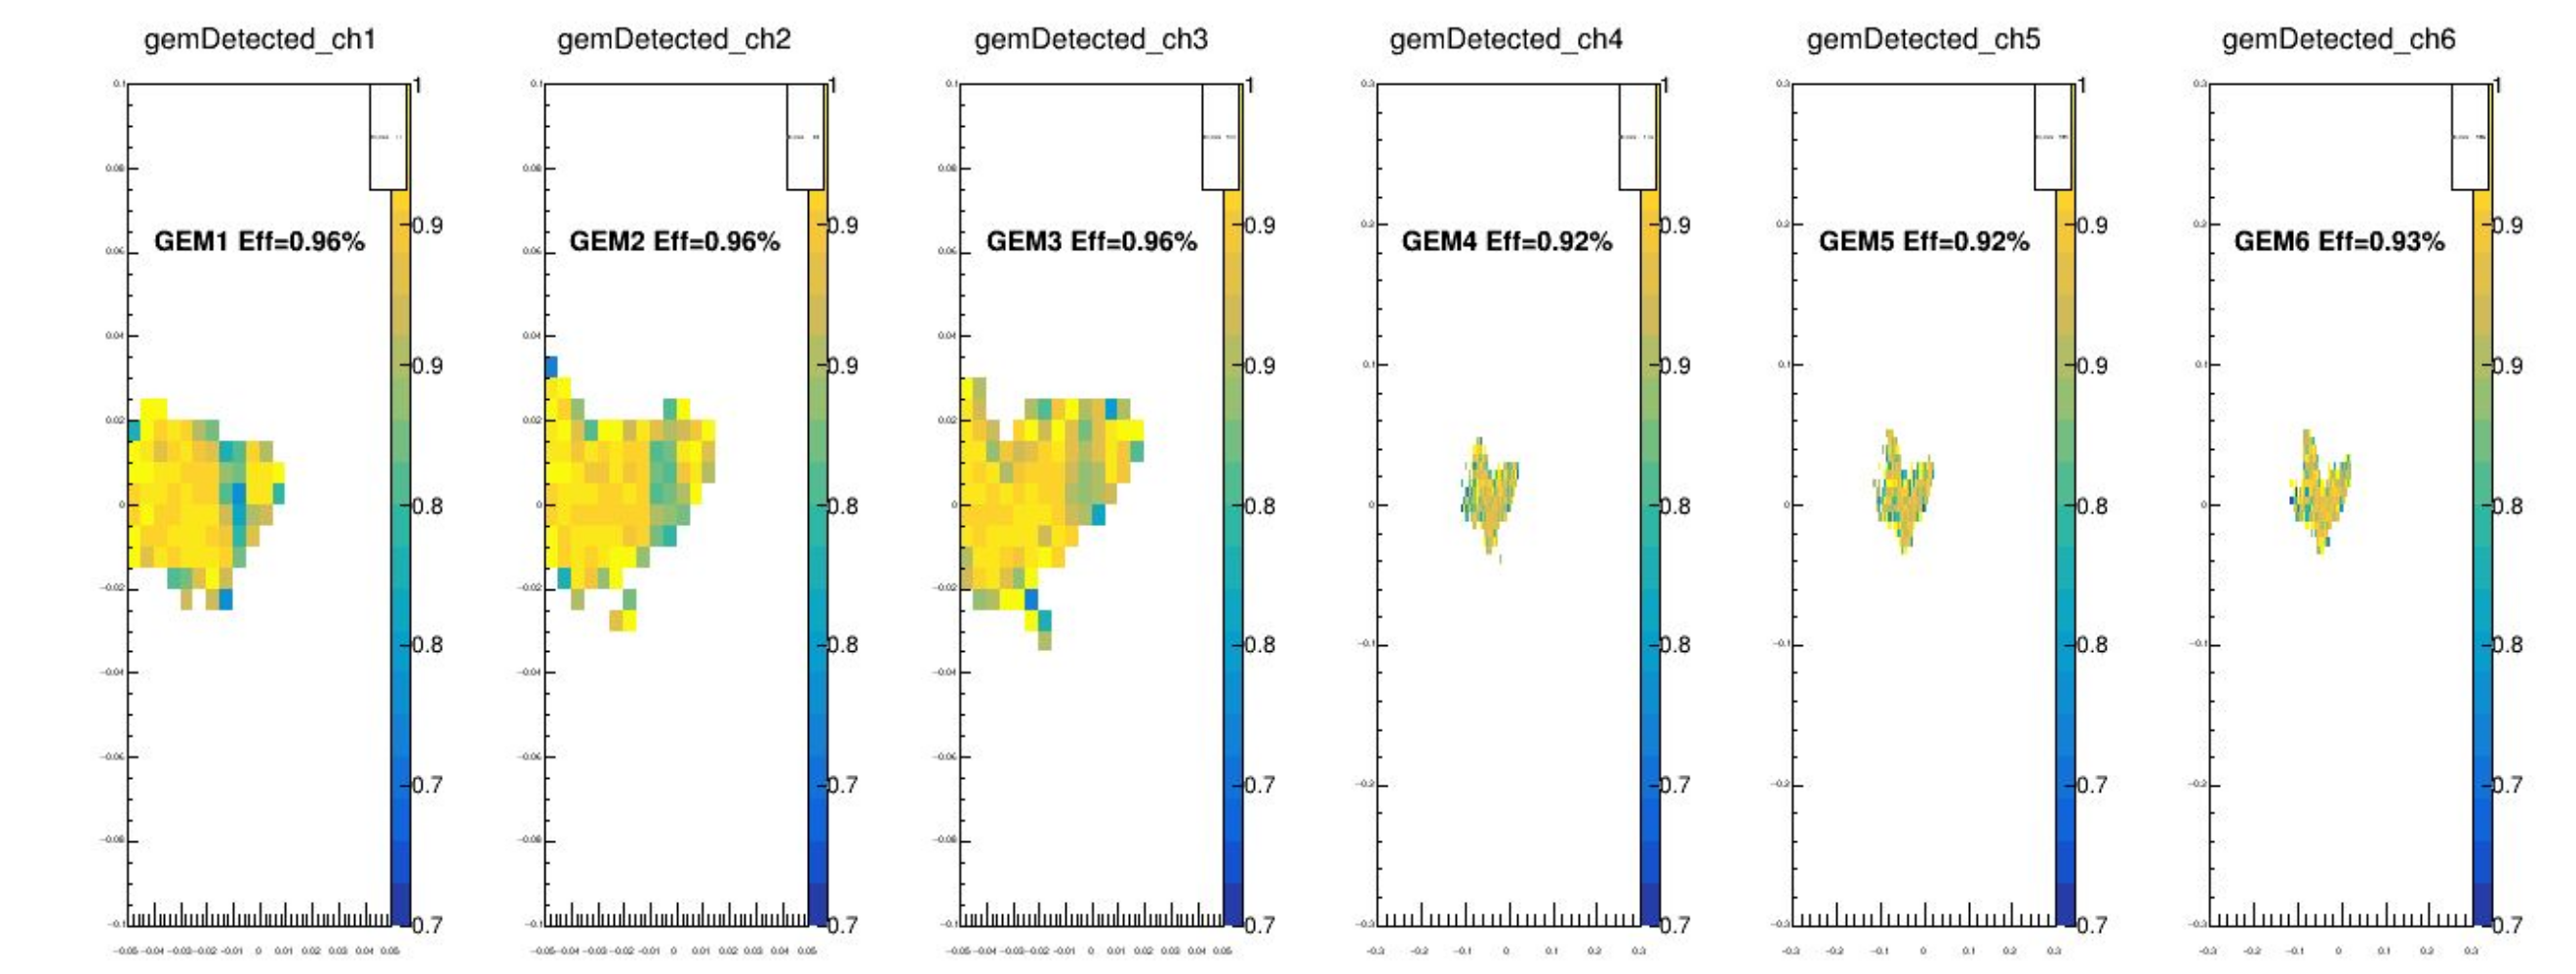
\includegraphics[width=\textwidth]{images/chap5/lhrs_efficiency_2d.png}
    \caption{Caption}
    \label{fig:my_label}
\end{figure}

\begin{figure}[!htbp]
    \centering
    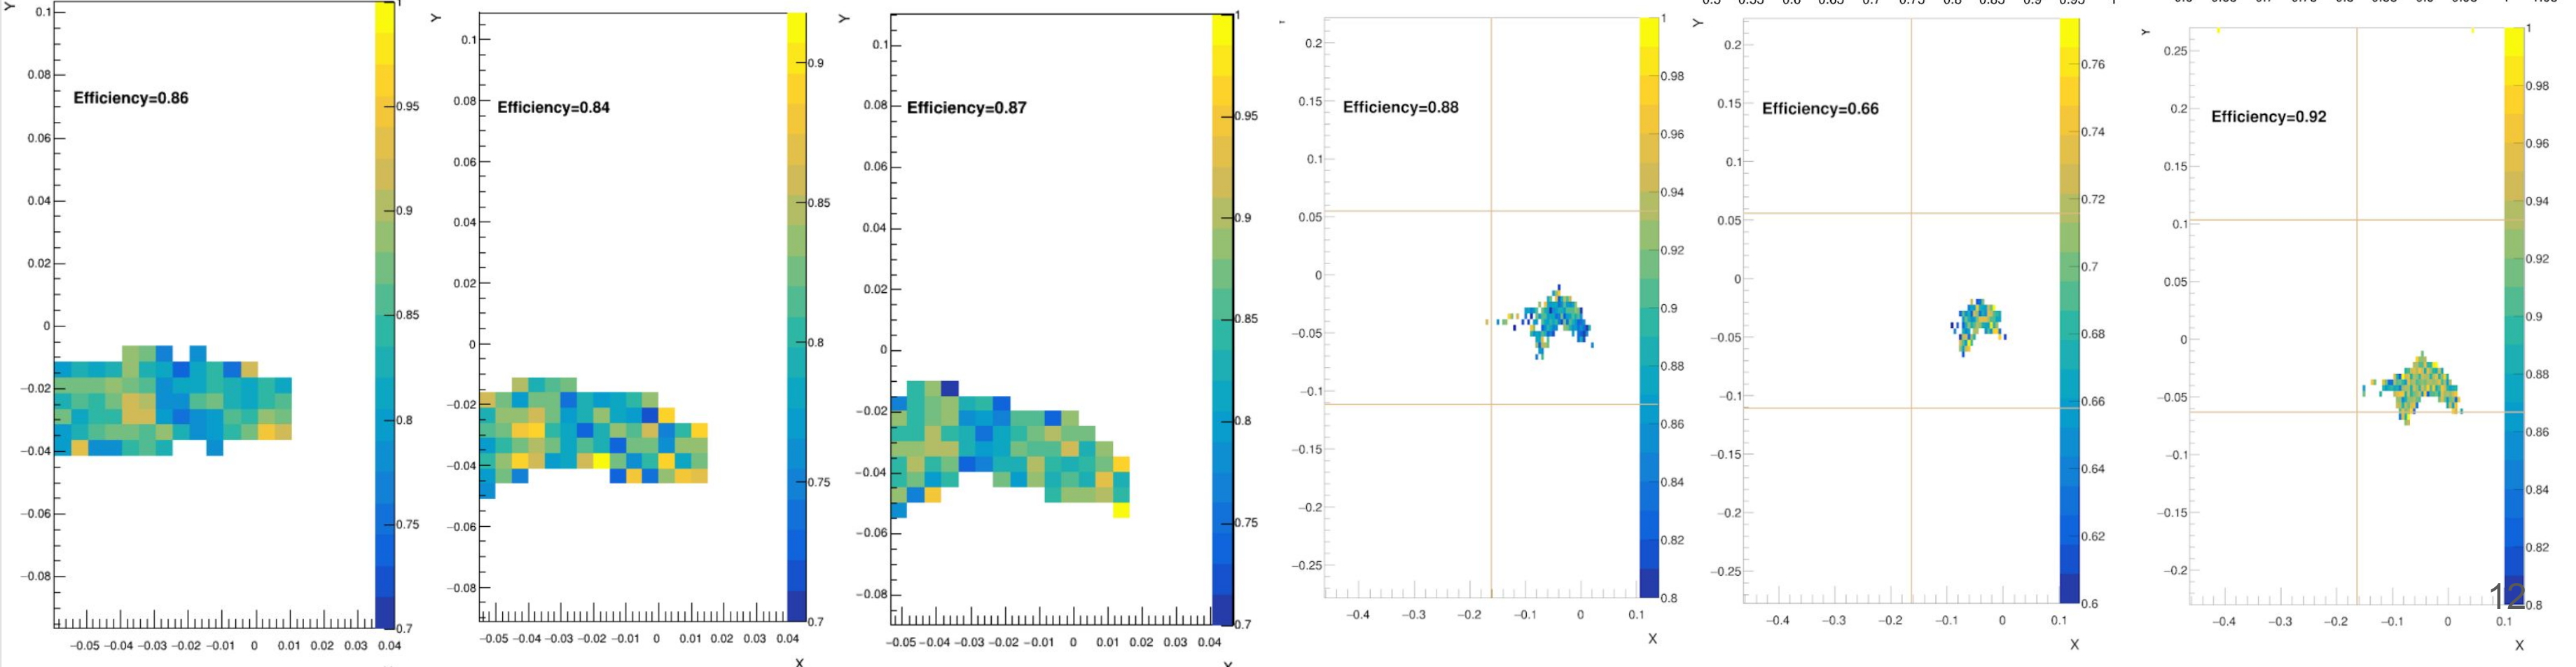
\includegraphics[width=\textwidth]{images/chap5/rhrs_efficiency_2d.png}
    \caption{Caption}
    \label{fig:my_label}
\end{figure}

\begin{figure}[!htbp]
    \centering
    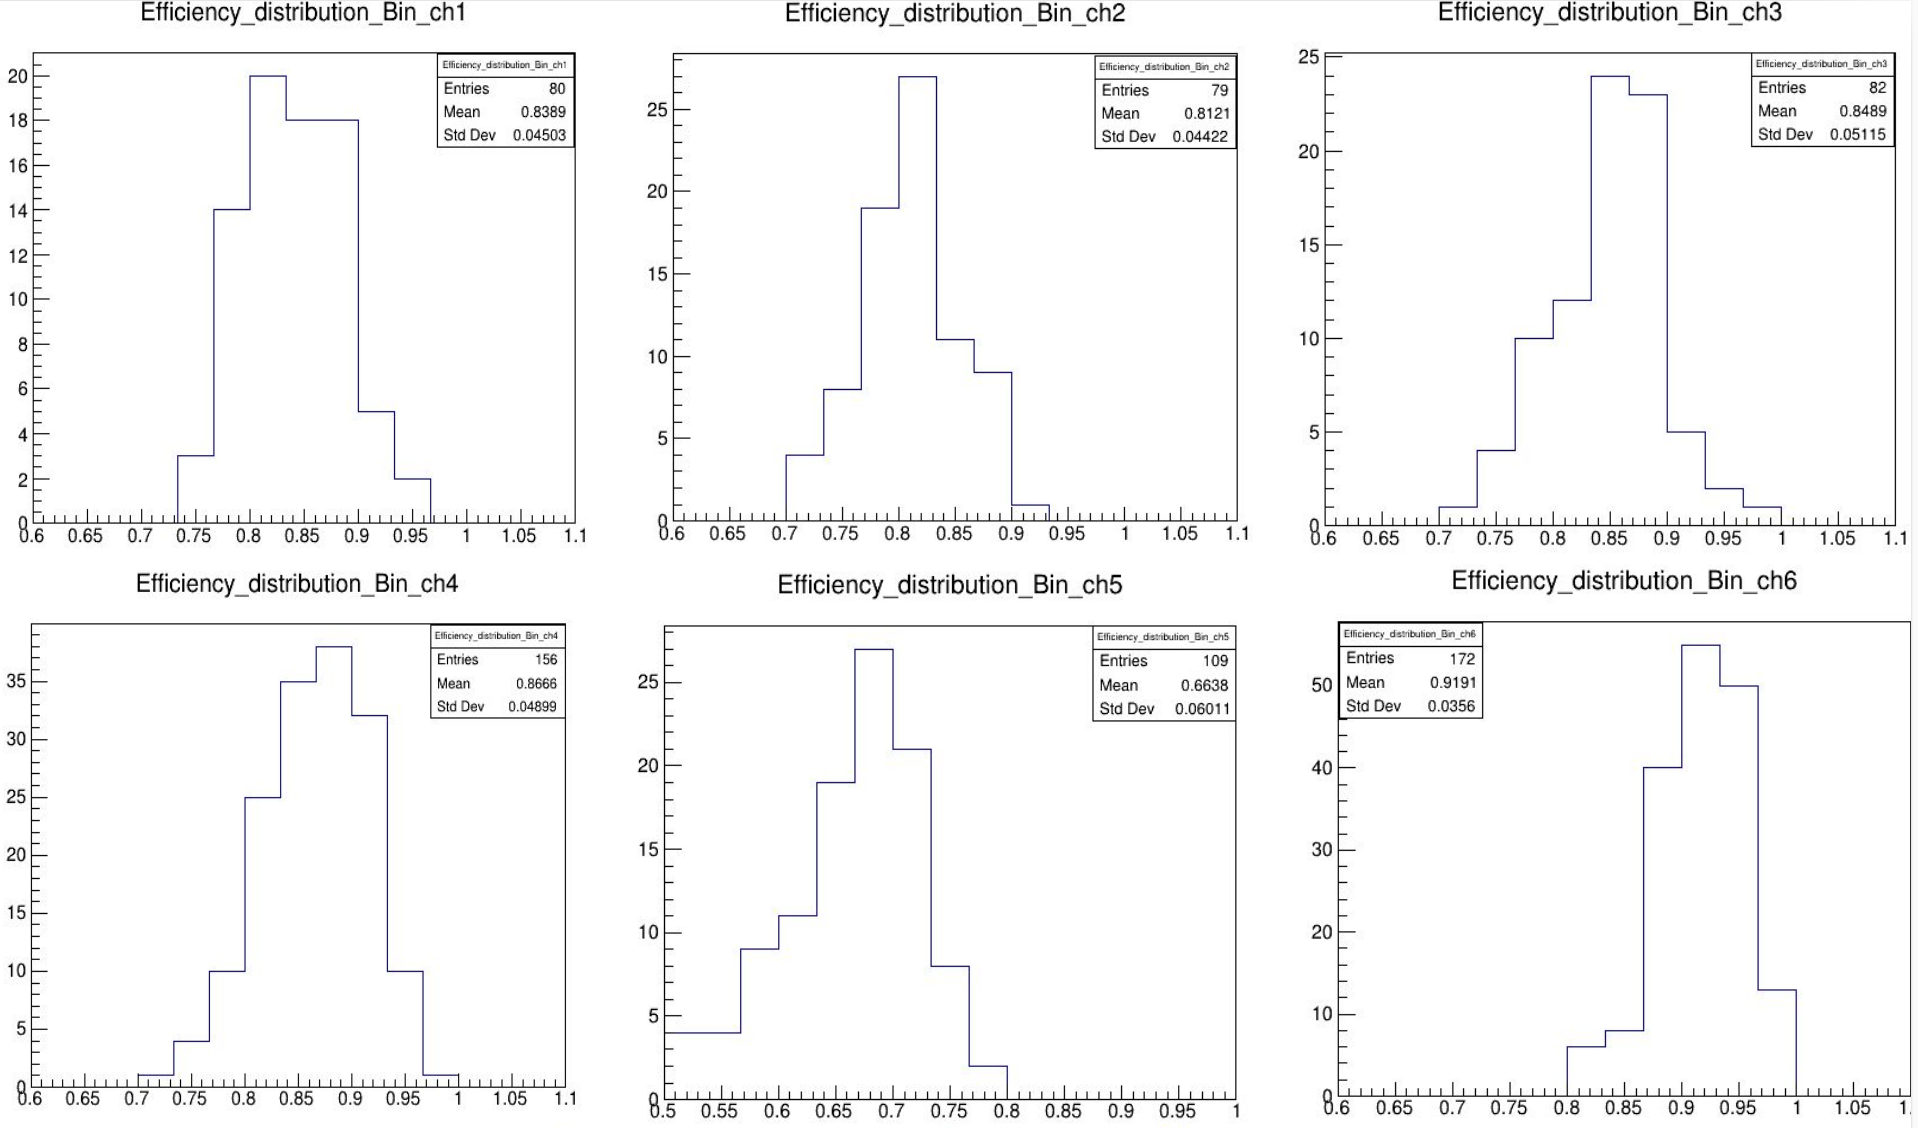
\includegraphics[width=\textwidth]{images/chap5/lhrs_gem_bin_efficiency.png}
    \caption{Caption}
    \label{fig:my_label}
\end{figure}

\begin{figure}[!htbp]
    \centering
    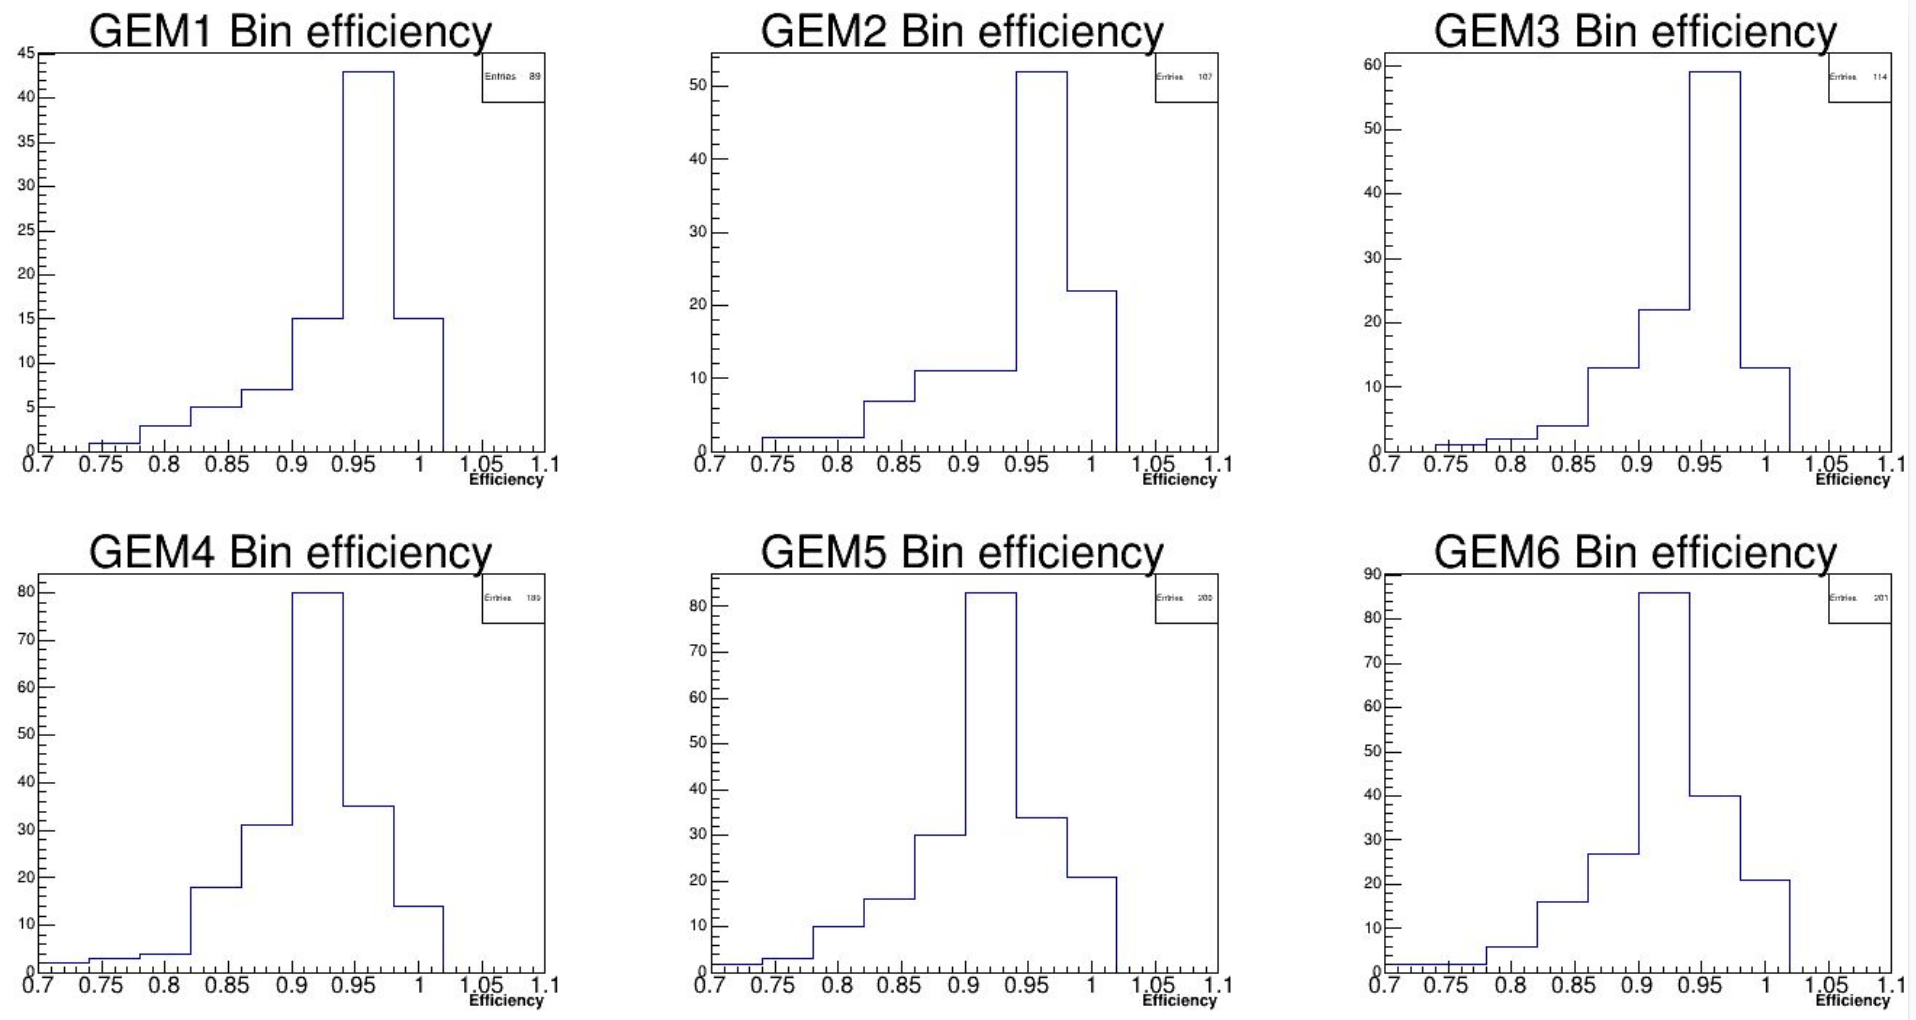
\includegraphics[width=\textwidth]{images/chap5/rhrs_gem_bin_efficiency.png}
    \caption{Caption}
    \label{fig:my_label}
\end{figure}


\begin{figure}[!htbp]
    \centering
    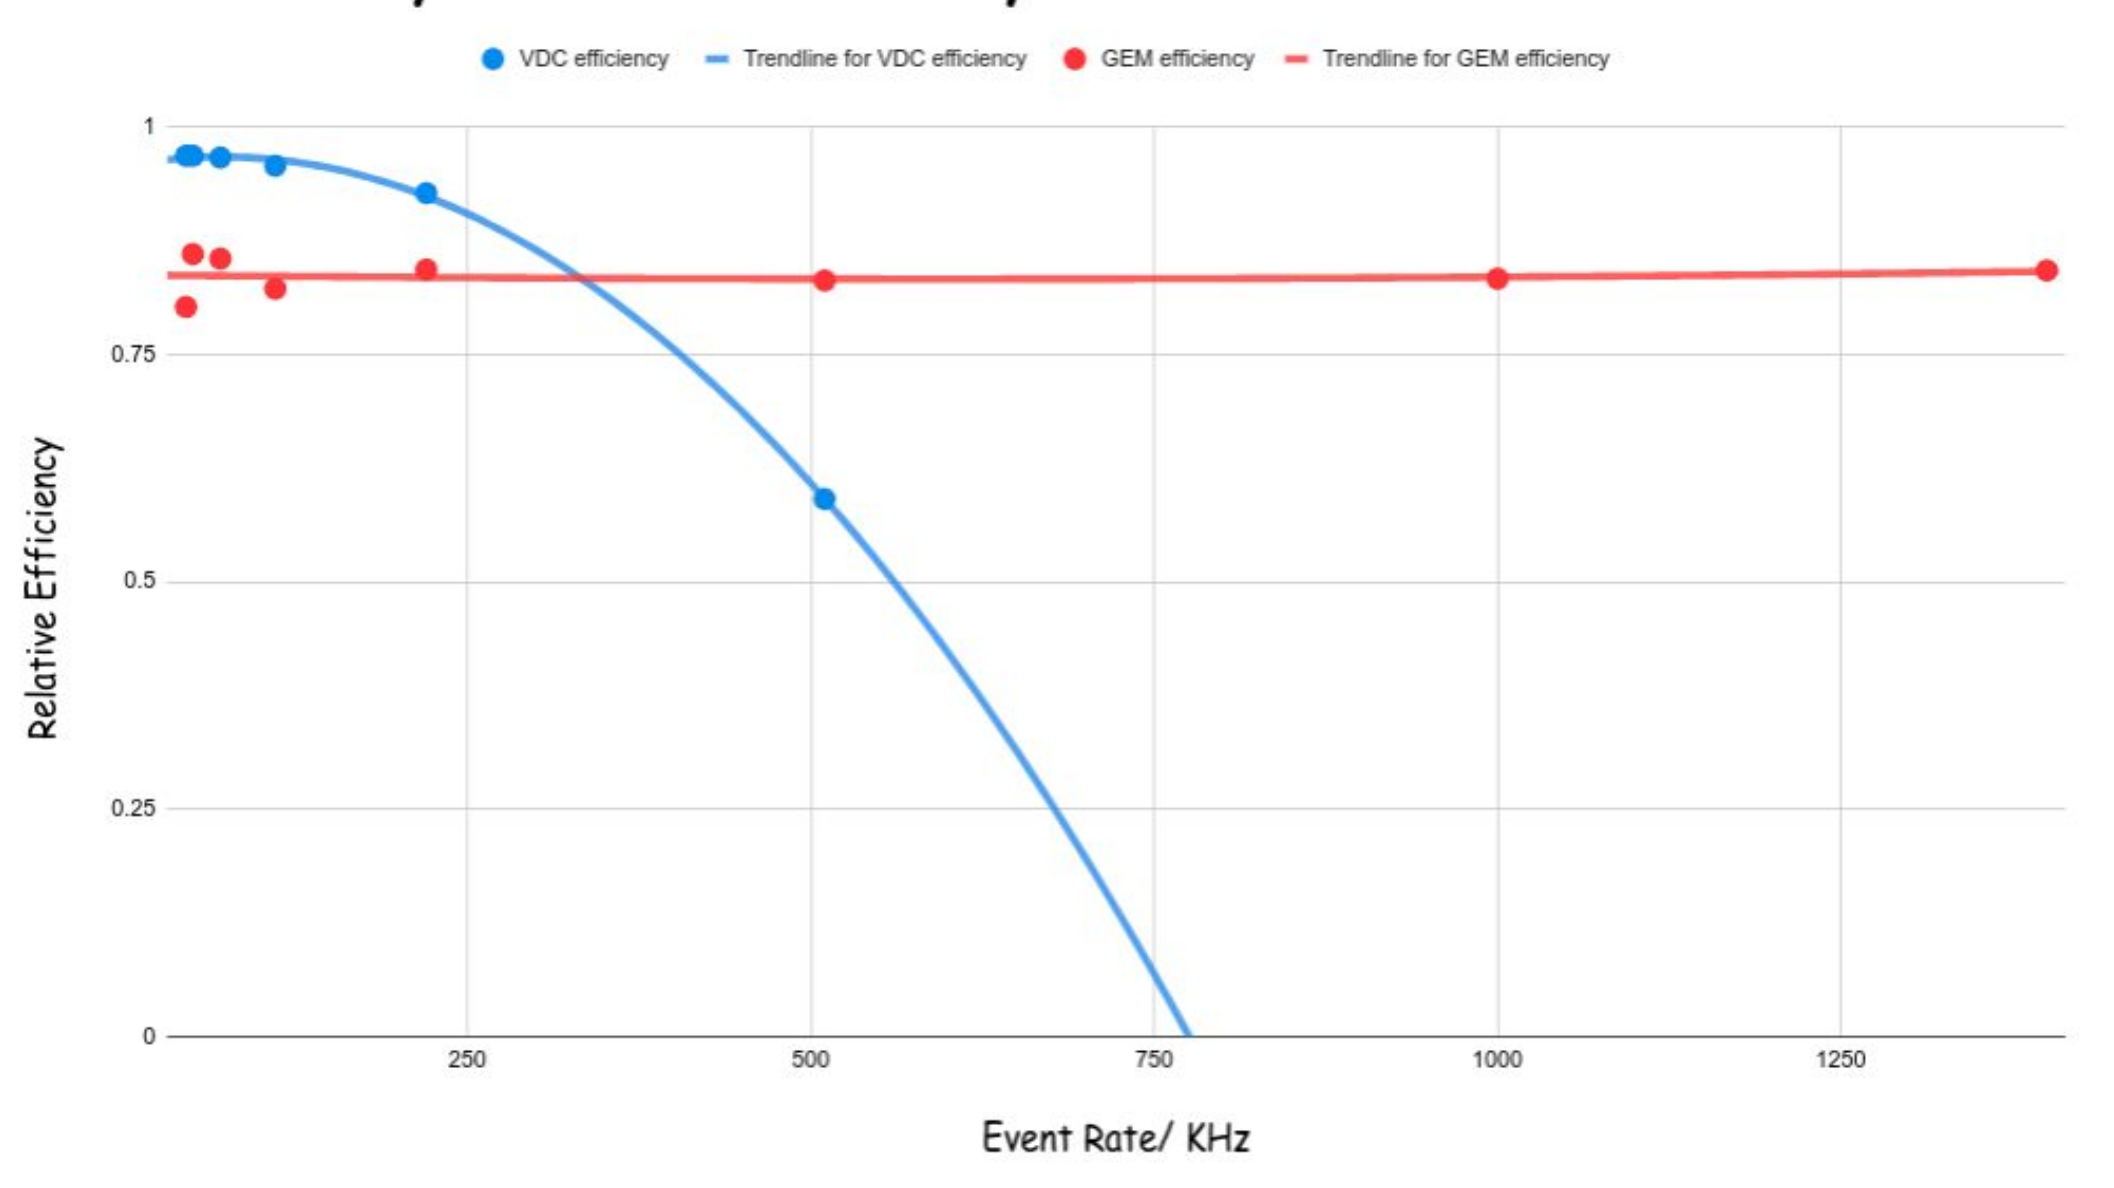
\includegraphics[width=\textwidth]{images/chap5/gem efficiency over time.png}
    \caption{Caption}
    \label{fig:my_label}
\end{figure}